\documentclass[14pt,a4paper,titlepage]{extarticle}
\usepackage[T2A,T1]{fontenc}
\usepackage[utf8]{inputenc}
\usepackage[ukrainian]{babel}
\usepackage{pgfplots}
\usepackage{hyperref}
\usepackage[margin=0.6in]{geometry}
\usepackage{setspace}

\setstretch{1.5}

\begin{document}

\begin{titlepage}
\setstretch{1}
\begin{center}
Міністерство освіти і науки України \\
Київський національний університет імені Тараса Шевченка \\
Кафедра обчислювальної математики факультету кібернетики

\vfill

\Large Випускна кваліфікаційна робота бакалавра \\
на тему \\
\LARGE Числові методи аналізу ДНК
\end{center}

\vfill

\begin{flushright}
Виконав студент 4-го курсу \\
Товт Аттіла Аттілович \\[1cm]

Науковий керівник \\
доктор фіз.-мат. наук, професор \\
Клюшин Дмитро Анатолійович
\end{flushright}

\center Київ 2015


\end{titlepage}

 \tableofcontents
 \newpage
\section{Вступ}
З розвитком біотехнологій все більше зразків послідовностей ДНК вдається
отримати. Кількість послідовностей росла експонентно на протязі минулих
двадцяти років. Послідовність ДНК складається з чотирьох різних нуклеотидів:
аденін(A), цитозин(C), гуанін(G) і тимін(T). Вона містить багато біологічної,
фізіологічної й хімічної інформації, через що стало дуже важливо аналізувати
генетичні послідовності. Було запропоновано багато обчислювальних і
статистичних методів для порівняння біологічних послідовностей. Не зважаючи на
це, тема порівняння послідовностей залишається актуальною і на цей час. Існуючі
методи можна розділити на групуючі і не групуючі. \par
Групуючі методи використовують динамічне програмування, за допомогою регресії знаходять оптимальне групування за допомогою присвоєння рахунку до різних можливих групувань і вибирають групування з найбільшим рахунком. \par
Серед всіх існуючих не групуючих методів порівняння біологічних послідовностей, графічне представлення забезпечує простий спосіб перегляду, сортування та порівняння генних структур. Мета графічного подання це відображення послідовності ДНК або білка графічно, так що ми можемо легко візуально визначити наскільки схожі або наскільки відрізняються послідовності. Звичайно, тільки візуального порівняння послідовностей недостатньо для подальшого дослідження. Потрібний більш точний спосіб порівняння. \par
У даній роботі будуть розглянуті основні методи представлення послідовності ДНК у числовому вигляді, а також спроба застосувати $p$-статистики як міри близькості між ними. Чисельні послідовності, які отримуються за допомогою одного з описаних нижче алгоритмів розглядаються як вибірки деякого неперервного розподілу. Далі ми використовуємо $p$-статистики, як міри близькості між розподілами.


\newpage
\section{Огляд літератури}
Описано багато методів числового представлення генетичних послідовностей. Тут ми розглянемо тільки ті, які здаються найбільш перспективними. У \cite{l1} розглядається наступний спосіб подання ДНК. Чотирьом нуклеотидам A, G, C і T ставляться у відповідність вектори: A $(1,0.8)$, G $(1,0.6)$, C $(1,0.4)$, T $(1,0.2)$. Елементи послідовності ми отримуємо, сумуючи вектори, що ставляться у відповідність нуклеотидам з послідовності.\par
\begin{figure}[h!]
\begin{center}
\begin{tikzpicture}
\begin{axis}[xmin=0,ymin=0]
\addplot[color=red,mark=x] coordinates {
(0,0)
(1.0, 0.8)
(2.0, 1.0)
(3.0, 1.6)
(4.0, 2.0)
(5.0, 2.2)
(6.0, 2.8)
(7.0, 3.2)
(8.0, 3.4)
(9.0, 4.0)
(10.0, 4.8)
};
\pgfplotsset{
after end axis/.code={
\node[black,above] at (axis cs:1,0.8){\small{$A$}};
\node[black,above] at (axis cs:2.0, 1.0){\small{$T$}};
\node[black,above] at (axis cs:3.0, 1.6){\small{$G$}};
\node[black,above] at (axis cs:4.0, 2.0){\small{$C$}};
\node[black,above] at (axis cs:5.0, 2.2){\small{$T$}};
\node[black,above] at (axis cs:6.0, 2.8){\small{$G$}};
\node[black,above] at (axis cs:7.0, 3.2){\small{$C$}};
\node[black,above] at (axis cs:8.0, 3.4){\small{$T$}};
\node[black,above] at (axis cs:9.0, 4.0){\small{$G$}};
\node[black,above] at (axis cs:10.0, 4.8){\small{$A$}};
}
}
\end{axis}
\end{tikzpicture}
\end{center}
\caption{Графічне представлення послідовності ATGCTGCTGA}
\label{fig:1}
\end{figure}
На Рис. \ref{fig:1} показано графічне представлення ДНК послідовності "ATGCTGCTGA". Таким чином ми отримуємо взаємно однозначну відповідність між послідовність нуклеотидів і отриманими точками.\par
Після цього у відповідність послідовності ДНК довжини $n$, ставиться у відповідність розподіл ймовірностей $(p_1,p_2,...,p_n)$,
\[{x_i-\overrightarrow{y_i} \over{{1\over2}n(n+1)-y_n}},\]
де $(x_i,y_i)$ відповідає позиції $i$-того нуклеотиду на графіку ДНК, $\overrightarrow{y_i}$ відповідає вибору $y$-координати при $i$-тому нуклеотиді у графічному представленні. Далі у цій статті доводиться, що це дійсно буде дискретним розподілом ймовірностей, а далі використовується розбіжність Кульбака-Лейблера або відносна ентропія.\par

У \cite{l2} описується метод графічного представлення послідовностей ДНК. Тут використовуються блукання у $2D$-просторі. Починають з точки $(0,0)$. Потім, в залежності від послідовності рухаємося у одному з чотирьох напрямків. Напрямки співвідносяться з нуклеотидами наступним чином: A=$(-1,0)$, G=$(1,0)$, C=$(0,1)$, T=$(0,-1)$. Зрозуміло, що блукаючи таким чином, точки будуть повторюватися, тому якщо ми потрапили в точку $m$ раз, ми присвоюємо їй вагу $m$. Для порівняння ДНК використовуються характеристики отриманих точок, такі як центр мас і тензори моменту інерції.\par

\begin{figure}[h!]
\begin{center}
\begin{tikzpicture}
\begin{axis}[xmin=0,xmax=1,ymin=0,ymax=1]
\addplot[color=red,mark=x] coordinates {
(0.5,0.5)
(0.25, 0.25)
(0.625, 0.125)
(0.8125, 0.5625)
(0.40625, 0.78125)
(0.703125, 0.390625)
(0.8515625, 0.6953125)
(0.42578125, 0.84765625)
(0.712890625, 0.423828125)
(0.8564453125, 0.7119140625)
(0.42822265625, 0.35595703125)
};
\pgfplotsset{
after end axis/.code={
\node[black,above] at (axis cs:0.25, 0.25){\small{$A$}};
\node[black,above] at (axis cs:0.62, 0.12){\small{$T$}};
\node[black,right] at (axis cs:0.81, 0.56){\small{$G$}};
\node[black,above] at (axis cs:0.40, 0.78){\small{$C$}};
\node[black,left] at (axis cs:0.70, 0.39){\small{$T$}};
\node[black,above] at (axis cs:0.85, 0.69){\small{$G$}};
\node[black,above] at (axis cs:0.42, 0.84){\small{$C$}};
\node[black,below] at (axis cs:0.71, 0.42){\small{$T$}};
\node[black,right] at (axis cs:0.85, 0.71){\small{$G$}};
\node[black,above] at (axis cs:0.42, 0.35){\small{$A$}};
}
}
\end{axis}
\end{tikzpicture}
\end{center}
\caption{Графічне представлення послідовності ATGCTGCTGA}
\label{fig:f2}
\end{figure}

У \cite{l3} використовуються нова область фізики, відома як, "нелінійна
динаміка", "хаотичні динамічні системи", або просто "хаос". Насправді, ця
ітеративна процедура з’явилася у статистичній механіці, зокрема в теорії хаосу.
Простір можна розглядати як безперервну систему посилань, в якій всі можливі
послідовності будь-якої довжини займають унікальне положення. Позиція
отримується за допомогою чотирьох можливих нуклеотидів, які розглядаються як
точки на квадраті зі стороною 1. Оскільки, формально генетичну послідовність
можна розглядати, як рядок складений з чотирьох літер A, C, G і T, то наступні
точки ставляться у відповідність чотирьом нуклеотидам: A=$(0,0)$, G=$(1,1)$,
C=$(0,1)$, T=$(1,0)$. Координати послідовності рахуються ітеративно, рухаючись
на половину відстані між попередньою позицією і точкою квадрата, якій
відповідає наступний нуклеотид у напрямку цієї точки. Наприклад, якщо G
наступний нуклеотид, то наступна точка буде по середині відрізка, що з’єднує
попередню точку і $(1,1)$. Ітеративну процедуру можна задати наступним чином:
\[p_i = p_{i-1}-0.5(p_{i-1}-g_i)\]
\[i=1,...,n; p_0=(0.5,0.5),\]
де $g_i$ - координати, що відповідають $i$-тому нуклеотиду, $n$ - довжина послідовності ДНК. На Рис. \ref{fig:f2} показано ламану утворену точками $p_i$ для послідовності "ATGCTGCTGA".\par
Кожній точці ставлять у відповідність число:
\[z_i = x_i + y_i,\]
де $x_i$, $y_i$ це $x$-координата і $y$-координата точки $p_i$. Далі розглядають чисельні характеристики послідовності $z_i$, зокрема середнє, часткове середнє, стандартне відхилення.

У \cite{l4} представленні методи кодування ДНК послідовностей у одновимірних,
двовимірних і тривимірних просторах. Основна ідея така сама, як в ітеративній
процедурі описаній у \cite{l3}. У $2D$-просторі алгоритми збігаються.
Відмінність тривимірного простору у тому, що тут нуклеотидам ставляться у
відповідність точки, що є вершинами тетраедра, а у одновимірному просторі
нуклеотидам T, G ставиться у відповідність $1$, а A, C ставиться у відповідність
$-1$.

У \cite{l5} вводиться поняття $p$-статистики, як міри близькості між
неперервними розподілами. У \cite{l6} це поняття розширюється на багатовимірні
розподіли, а у \cite{l7} вводиться модифікована $p$-статистика, яку можна
застосовувати до вибірок з повтореннями.

\newpage
\section{Постановка задачі}
Використовуючи відомі алгоритми числового представлення послідовності ДНК, знайти такі, які допускають використання $p$-статистик. Перевірити доцільність застосування $p$-статистик до знайдених алгоритмів шляхом порівняння за допомогою них послідовностей ДНК різних видів. Послідовності ДНК можна взяти з ГенБанку(www.ncbi.nlm.nih.gov/genbank/).

\section{Алгоритм розв’язання}
Подаємо відрізок ДНК у вигляді числової послідовності, за допомогою одного з
методів описаного нижче. Вважаємо, що отримана числова послідовність є вибіркою,
якогось неперервного розподілу і, використовуючи $p$-статистики, порівнюємо
вибірки отримані з геномних послідовностей різних видів.

\subsection{Методи числового подання ДНК}

\paragraph{Метод 1}
Кожному нуклеотиду A, G, C, T ставимо у відповідність вектори $(1,0.8)$, $(1,0.6)$, $(1,0.4)$, $(1,0.2)$. Починаючи з точки $(0,0)$ рухаємось у напрямку векторів. Точки через які ми проходимо утворюють послідовність.
\paragraph{Метод 2}
Спочатку використаємо попередній метод щоб отримати числову послідовність $(x_i,y_i)$. Далі використаємо наступну формулу для обчислення результуючої послідовності:
\[{x_i-\overrightarrow{y_i} \over{{1\over2}n(n+1)-y_n}},\]
де $\overrightarrow{y_i}$ це $y$-компонента вектора, що відповідає $i$-тому нуклеотиду при використанні методу 1, $n$ це розмір ДНК послідовності.
\paragraph{Метод 3}
Нуклеотидам A, G, C, T ставимо у відповідність вектори $(-1,0)$, $(1,0)$, $(0,1)$, $(0,-1)$. Починаємо з точки $(0,0)$ і рухаємось по відповіднім векторам. Точки через які ми проходимо утворюють послідовність, причому точка стільки разів зустрічається у послідовності, скільки разів ми в неї потрапили.
\paragraph{Метод 4}
Розташовуємо нуклеотиди у вершинах квадрата зі стороною 1: A=$(0,0)$, G=$(1,1)$, C=$(0,1)$, T=$(1,0)$. Координати послідовності рахуються ітеративно, рухаючись на половину відстані між попередньою позицією і точкою квадрата, якій відповідає наступний нуклеотид у напрямку цієї точки. Ітеративну процедуру можна задати наступним чином:
\[p_i = p_{i-1}-0.5(p_{i-1}-g_i)\]
\[i=1,...,n; p_0=(0.5,0.5),\]
де $g_i$ - координати, що відповідають $i$-тому нуклеотиду, $n$ - довжина послідовності ДНК.
\paragraph{Метод 5}
Використовуємо попередній метод, щоб отримати послідовність $p_i$, отримуємо результуючу, як суму всіх попередніх:
\[z_i = \sum_{j=1}^{i} p_i\]
\paragraph{Метод 6}
Отримуємо за допомогою методу 4 послідовність $p_i$ і, щоб отримати результуючу послідовність, кожній точці ставимо у відповідність число:
\[z_i = x_i + y_i,\]
де $p_i = (x_i,y_i)$.
\paragraph{Метод 7}
Нуклеотидам A,C ставимо у відповідність $-1$, а нуклеотидам T,G ставимо у відповідність $1$. Починаючи з точки $0$ рухаємось ітеративно:
\[p_i = p_{i-1} - {(g_i-p_{i-1}) \over{2}}sign(g_i)\]
де $g_i$ число яке відвідає $i$-тому нуклеотиду. Тобто ми, подібно до методу 4, рухаємося на пів відстань до числа яке відповідає $i$-тому нуклеотиду.

\subsection{$p$-статистики}


Позначимо через $H$ гіпотезу про рівність неперервних функцій
розподілу  $F_G(u)$ і $F_{G'}(u)$ генеральних сукупностей $G$ і $G'$ відповідно.
Нехай $x=(x_1,...,x_n)\in G$ і $x'=(x_1',...,x_m')\in G'$, $x_{(1)}<...<x_{(n)}$, $x_{(1)}'<...<x_{(n)}'$ - порядкові статистики.
Припустимо, що $F_G(u) = F_{G'}(u)$. Позначимо через $A_{ij}^{(k)}$, $k=1,2,..., m$
випадкову подію, яка полягає в тому, що $x_k'$ потрапляє в інтервал  $\left(x_{(i)},x_{(j)}\right)$,
тобто $A_{ij}^{(k)} = \left\{x_k' \in \left(x_{(i)}, x_{(j)}\right)\right\}$. Якщо $F_G(u) = F_{G'}(u)$ (тобто $G = G'$) імовірність
цієї події обчислюється за формулою:
\[P\left(A_{ij}^{(k)}\right) = P\left(x_k' \in \left(x_{(i)}, x_{(j)}\right)\right) = p_{ij}^{(n)} = {{j-i}\over{n+1}} = {{q}\over{n+1}}, q = j-i\]
Покладемо
\begin{equation}\label{eq:p1}
p_{ij}^{(1)} = {{h_{ij}^{(n)}m+g^2/2-g\sqrt{h_{ij}^{(n)}(1-h)m+g^2/4}}\over{m+g^2}},
\end{equation}
\begin{equation}\label{eq:p2}
p_{ij}^{(2)} = {{h_{ij}^{(n)}m+g^2/2+g\sqrt{h_{ij}^{(n)}(1-h)m+g^2/4}}\over{m+g^2}},
\end{equation}
де $h_{ij}^{(n)}$ — частота події $A_{ij}^{(n)}$
в $m$ випробуваннях. Величина $g$ визначає
рівень значущості довірчого інтервалу $I_{ij}^{(n,m)} = \left(p_{ij}^{(1)},p_{ij}^{(2)}\right)$; в силу правила $3\sigma$
при $g=3$ рівень значущості цього інтервалу не перевищує $0.05$.
\par
Позначимо через $N$ кількість всіх довірчих інтервалів
$I_{ij}^{(n,m)} = \left(p_{ij}^{(1)},p_{ij}^{(2)}\right)$ ($N=n(n-1)/2$) і $L$ -
кількість тих інтервалів $I_{ij}^{(n,m)}$, які містять ймовірності $p_{ij}^{(n)}$. Покладемо $h^{(n,m)}=\rho \left(F^{*},{F^{*'}}\right) = \rho(x,x') = {L\over{N}}$.
Оскільки $h^{(n,m)}$ –
частота випадкової події $B=\left\{p_{ij}^{(n)} \in I_{ij}^{(n,m)}\right\}$, що має імовірність $p(B)=1-\beta$,
то, покладаючи в формулі $h_{ij}^{(n,m)} = h^{(n)}, m = N$ і $g=3$ , ми отримаємо
довірчий інтервал $I^{(n,m)} = \left(p^{(1)},p^{(2)}\right)$ для імовірності
$p(B)$. Статистику $h^{(n)}$
називатимемо $p$-статистикою. Вона є мірою близькості  $\rho(x,x')$ між вибірками
$x$ і $x'$.

\subsection{Модифікована $p$-статистика}
%Тепер введемо поняття модифікованої $p$-статистики.\par
Нехай $x=(x_1, x_2,...,x_n)$ — вибірка, отримана з генеральної
сукупності $G$, що має функцію розподілу $F(u)$ , за допомогою простого
випадкового вибору. Атомом вибірки $x$ будемо називати вибіркове
значення $x_k$ , що зустрічається у вибірці $x$ більше одного разу:
$x_k=x_{k_1}=...=x_{k_i}, k,k_1,...,k_i \in \{1,2,...,n\}$.
Кратністю $t(x_k)$ довільного
вибіркового значення $x_k$ називатимемо кількість його повторень у
виборці $x$. Таким чином, атоми — це вибіркові значення, кратність яких
перебільшує одиницю. \par
Нехай $x_{(1)}\leq ... \leq x_{(n)}$ - варіаційний ряд вибірки $x$.
Тоді згідно \cite{l7}:
\begin{equation}\label{eq:p_ij}
p_{ij}=p\left(A_{ij}\right)=p\left(x^{*} \in (x_{(i)}, x_{(j)})\right) \approx
\gamma_i + \gamma_{i+1} + ... + \gamma_{j-1} + {{j-i}\over{n+1}},
\end{equation}
\[\gamma_{l} = \gamma \left(x_{(l)}\right) = {{t(x_{(k)})-1}\over{n+1}},\]
де $x^{*}$ вибіркове значення із генеральної сукупності $G$ , що не
залежить від вибірки $x$.\par

Позначимо через $H$ гіпотезу про рівність неперервних функцій
розподілу  $F_G(u)$ и $F_{G'}(u)$ генеральних сукупностей $G$ і $G'$ відповідно.
Нехай $x=(x_1,...,x_n)\in G$ і $x'=(x_1',...,x_m')\in G'$, $x_{(1)} \leq ... \leq x_{(n)}$, $x_{(1)}' \leq ... \leq x_{(n)}'$ - порядкові статистики.
Причому, вибірки $x$ і $x'$ містять атоми.
Припустимо, що $F_G(u) = F_{G'}(u)$. Позначимо через $A_{ij}^{(k)}$, $k=1,2,..., m$
випадкову подію, яка полягає в тому, що $x_k'$ потрапляє в інтервал  $\left(x_{(i)},x_{(j)}\right)$,
тобто $A_{ij}^{(k)} = \left\{x_k' \in \left(x_{(i)}, x_{(j)}\right)\right\}$. Якщо $F_G(u) = F_{G'}(u)$ (тобто $G = G'$) імовірність
цієї події обчислюється за формулою \ref{eq:p_ij}.\par
За формулами \ref{eq:p1} і \ref{eq:p2} обчислюємо $p_{ij}^{(1)}$ і $p_{ij}^{(2)}$, відповідно.
Позначимо через $N$ кількість всіх довірчих інтервалів
$I_{ij}^{(n,m)} = \left(p_{ij}^{(1)},p_{ij}^{(2)}\right)$ ($N=n(n-1)/2$) і $L$ -
кількість тих інтервалів $I_{ij}^{(n,m)}$, які містять ймовірності $p_{ij}^{(n)}$. Покладемо $h^{(n,m)}=\rho \left(F^{*},{F^{*'}}\right) = \rho(x,x') = {L\over{N}}$.
Оскільки $h^{(n,m)}$ –
частота випадкової події $B=\left\{p_{ij}^{(n)} \in I_{ij}^{(n,m)}\right\}$, що має імовірність $p(B)=1-\beta$,
то, покладаючи в формулі $h_{ij}^{(n,m)} = h^{(n)}, m = N$ і $g=3$ , ми отримаємо
довірчий інтервал $I^{(n,m)} = \left(p^{(1)},p^{(2)}\right)$ для імовірності
$p(B)$. Статистику $h^{(n)}$ називатимемо модифікованою $p$-статистикою.


\subsection{Еліпсоїд Петуніна}
Розглянемо множину двовимірних точок $M_n$:
\[M_n = \left\{\overrightarrow{x_1},...,\overrightarrow{x_n}\right\},
де \overrightarrow{x_i} = (x_i, y_i)\]

\begin{figure}[h!]
\centering
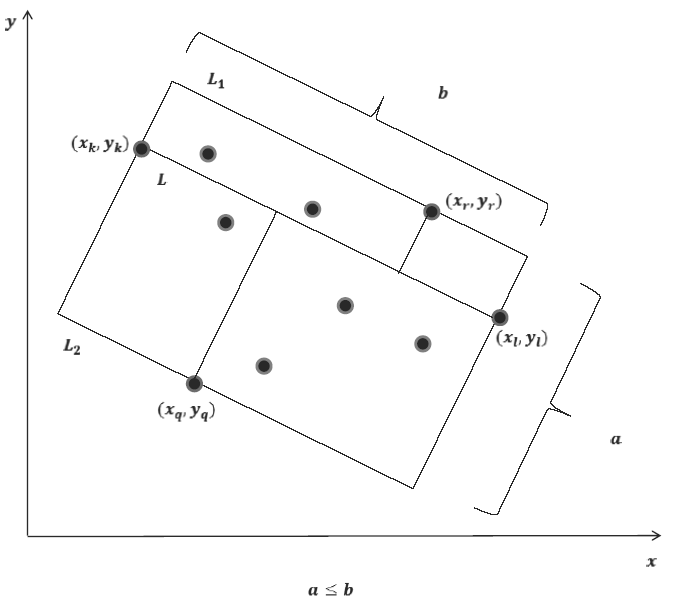
\includegraphics[width=0.65\textwidth]{pet1}
\caption{Прямокутник Петуніна}
\label{fig:pet1}
\end{figure}

Побудуємо опуклу оболонку точок $M_n = \left\{(x_1,y_1),...,(x_n,y_n)\right\}$.
Знайдемо вершини опуклої оболонки $(x_k,y_k)$ і $(x_l,y_l)$,
які лежать на діаметрі опуклої оболонки,
тобто найбільш віддалені одна від одної вершини.
З’єднаємо точки $(x_k,y_k)$ і $(x_l,y_l)$ відрізком $L$.
Знайдемо вершини $(x_r,y_r)$ і $(x_q,y_q)$ опуклої оболонки
найбільш віддалені від $L$.
З’єднаємо точки $(x_r,y_r)$ і $(x_q,y_q)$ відрізками паралельними
$L_1$ і $L_2$, паралельними відрізку $L$.
Проведемо через точки $(x_k,y_k)$ і $(x_l,y_l)$ відрізки $L_3$ і $L_4$,
перпендикулярно до відрізка $L$. Перетин відрізків $L_1$, $L_2$, $L_3$ і $L_4$
утворюють прямокутник $\Pi$, сторони якого мають довжину $a$ і $b$.(Рис.
\ref{fig:pet1})
\par

Будемо вважати, що $a \leq b$. Переведемо лівий нижній кут прямокутника у
початок нової системи координат з осями $Ox'$ і $Oy'$ за допомогою паралельного
переносу і повороту. Точки $(x_1,y_1), (x_2,y_2),...,(x_n,y_n)$ перейдуть в
точки$(x_1',y_1'), (x_2',y_2'),...,(x_n',y_n')$. Відобразимо точки
$(x_1',y_1'), (x_2',y_2'),...,(x_n',y_n')$ в точки $(\alpha x_1',y_1'), (\alpha
x_2',y_2'),...,(\alpha x_n',y_n')$, де $\alpha = {a\over{b}}$. В результаті
отримаємо сукупність точок, які належать квадрату $S$. \par

Порахуємо центр $(x_0',y_0')$ квадрата $S$ і знайдемо відстані
$r_1,r_2,...,r_n$ від нього до кожної точки $(\alpha x_1',y_1'), (\alpha
x_2',y_2'),...,(\alpha x_n',y_n')$. Найбільше число $R=max(r_1,r_2,...,r_n)$
визначає круг з центром у точці $(x_0',y_0')$ і радіусом $R$.\par
В результаті всі
точки $(\alpha x_1',y_1'), (\alpha x_2',y_2'),...,(\alpha x_n',y_n')$ всередині
круга з радіусом $R$. Розтягуючи цей круг вздовж осі $Ox'$ з коефіцієнтом
$\beta={1\over \alpha}$ і виконуючи обернені перетворення повороту і переносу,
отримаємо еліпс Петуніна (Рис. \ref{fig:pet2}).\par

\begin{figure}[h!]
\centering
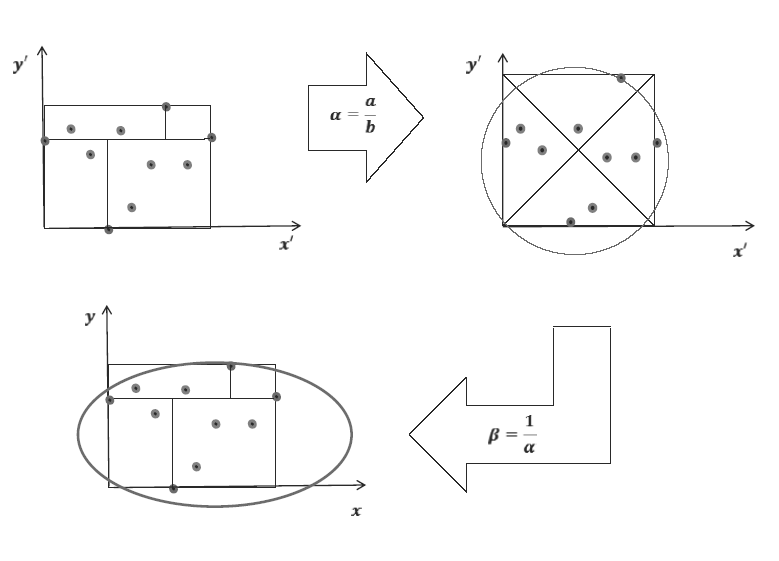
\includegraphics[width=0.75\textwidth]{pet2}
\caption{Побудова еліпса Петуніна}
\label{fig:pet2}
\end{figure}

\begin{figure}[h!]
\centering
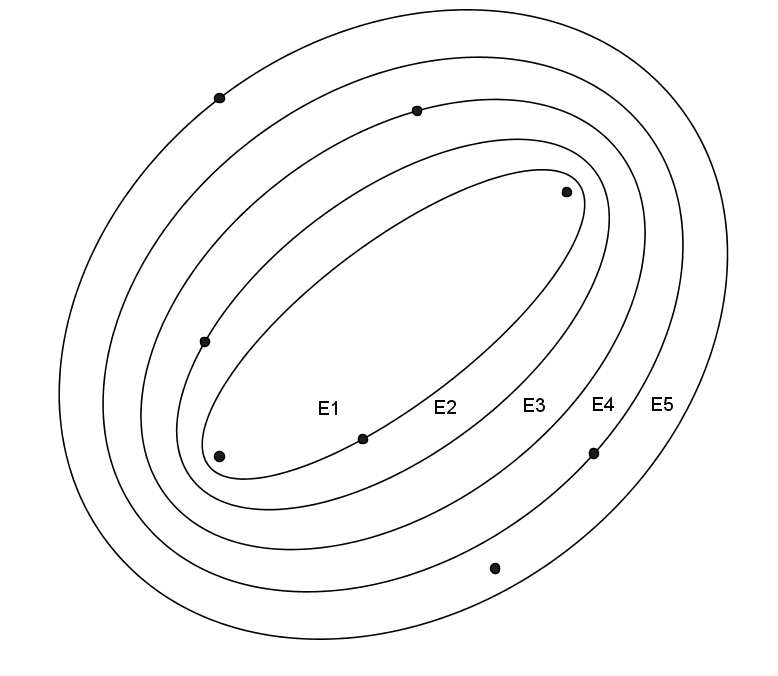
\includegraphics[width=0.5\textwidth]{pet3}
\caption{Вкладені еліпси Петуніна}
\label{fig:pet3}
\end{figure}

У $m$-вимірному просторі на першому кроці знайдемо вершини опуклої оболонки
$\overrightarrow{x_k}$ і $\overrightarrow{x_l}$, що лежать на діаметрі випуклої
оболонки. З’єднаємо точки $\overrightarrow{x_k}$ і $\overrightarrow{x_l}$
відрізком $L$. Повернемо і перенесемо систему координат, щоб діаметр опуклої
оболонки лежав на осі $Ox_1'$. Побудуємо найменший прямокутний паралелепіпед,
що містить точки $\overrightarrow{x_1},...,\overrightarrow{x_n}$.
\par

Зжимаючи прямокутний паралелепіпед, Відобразимо точки у гіперкуб. Знайдемо
центр $\overrightarrow{x_0}$ гіперкуба і порахуємо відстані $r_1,r_2,...,r_n$
від нього до кожної точки. Знайдемо найбільше число $R=max(r_1,r_2,...,r_n)$ і
побудуємо гіперкулю з центром в точці $\overrightarrow{x_0}$ і радіусом $R$.
Застосовуючи до цієї гіперкулі обернені операції розтягування, повороту і
переносу, отримаємо еліпсоїд Петуніна в $m$-вимірному просторі.
\par

Якщо побудувати серію вбудованих еліпсоїдів, то на кожному з них буде лежати по одній точці, тобто відбувається їх ранжування (Рис. \ref{fig:pet3}).

\par

При побудові $p$-статистики варіаційному ряду вибірок
$\overrightarrow{x}_{(1)} \preceq \overrightarrow{x}_{(2)} \preceq
... \preceq \overrightarrow{x}_{(n)}$ поставимо у відповідність послідовність
вкладених еліпсоїдів $E_{(1)} \subset E_{(2)} \subset ... \subset E_{(n)}$. Ймовірність того, що елемент $\overrightarrow{x}$ із генеральної сукупності $G$ задовольняє умові $\overrightarrow{x}_{(i)} \preceq \overrightarrow{x} \preceq
\overrightarrow{x}_{(j)}$, рівна ймовірності потрапити між еліпсами $E_{(i)}$ і $E_{(j)}$, тобто $j-i \over n+1$. Ця умова дозволяє побудувати $p$-статистику для багатовимірного випадку. \par
Таким чином будуємо $p$-статистику як завжди, тільки подія $A_{ij}^{(k)}$ буде полягати в тому, що $x_k'$ попаде в область $E_{(j)} \setminus E_{(i)}$.

\newpage

\section{Результати}
Нижче представлені результати застосування одного з методів числового представлення ДНК і $p$-статистик.\par
В таблицях представлені результати, порівнюючи послідовностей ДНК джунглевих
кур(gallus), пацюка(rat), кролика(rabbit), людини(human), качки(duck) і
горили(gorilla).\par
Геномні послідовності були взяті з ГенБанку (www.ncbi.nlm.nih.gov/genbank/):\par
(gi|126165289|ref|NM\_001081704.1| Gallus gallus hemoglobin, beta (HBE), mRNA),\par
rat(gi|56251|emb|X06701.1| Rat beta-globin gene),\par
rabbit(gi|1489|emb|V00882.1| Rabbit (O. cuniculus) gene for beta-globin),\par
human(gi|34190730|gb|BC047343.2| Homo sapiens cDNA clone IMAGE:5177205),\par
duck(gi|483525371|gb|KB742400.1| Anas platyrhynchos breed Pekin duck unplaced genomic scaffold scaffold30, whole genome shotgun sequence),\par
gorilla(gi|401612384|ref|NW\_004008464.1| Gorilla gorilla gorilla unplaced genomic scaffold, gorGor3.1 Primary Assembly unplaced10718\_1\_913, whole genome shotgun sequence)\par

\newpage
\begin{table}[h!]
\begin{center}
\begin{tabular}{|c|c|c|c|c|c|c|}
\hline
- & gallus & rat & rabbit & human & duck & gorilla \\ \hline
gallus & - & 0.0089988408 & 0.00899884 & 0.00450450 & 0.01364569 & 0.01810953 \\ \hline
rat & - & - & 0.00869077 & 0.00633129 & 0.00797394 & 0.00879594 \\ \hline
rabbit & - & - & - & 0.00618809 & 0.00996201 & 0.01100094 \\ \hline
human & - & - & - & - & 0.00595238 & 0.00441478 \\ \hline
duck & - & - & - & - & - & 0.01754385 \\ \hline
gorilla & - & - & - & - & - & - \\ \hline
\end{tabular}
\end{center}
\caption{$p$-статистики при представленні ДНК методом 1}
\label{table:res1}
\end{table}

\begin{table}[h!]
\begin{center}
\begin{tabular}{|c|c|c|c|c|c|c|}
\hline
- & gallus & rat & rabbit & human & duck & gorilla \\ \hline
gallus & - & 0.0322127997 & 0.03896447 & 0.01770280 & 0.07635287 & 0.09231692 \\ \hline
rat & - & - & 0.30298690 & 0.07789030 & 0.06677661 & 0.05957562 \\ \hline
rabbit & - & - & - & 0.05915402 & 0.09385886 & 0.08013153 \\ \hline
human & - & - & - & - & 0.03564335 & 0.03172258 \\ \hline
duck & - & - & - & - & - & 0.72325906 \\ \hline
gorilla & - & - & - & - & - & - \\ \hline
\end{tabular}
\end{center}
\caption{$p$-статистики при представленні ДНК методом 2}
\label{table:res2}
\end{table}

\newpage

\begin{table}[h!]
\begin{center}
\begin{tabular}{|c|c|c|c|c|c|c|}
\hline
- & gallus & rat & rabbit & human & duck & gorilla \\ \hline
gallus & - & 0.0183905103 & 0.01839051 & 0.00921658 & 0.02752176 & 0.04045058 \\ \hline
rat & - & - & 0.03392735 & 0.01003638 & 0.02044937 & 0.01820214 \\ \hline
rabbit & - & - & - & 0.01050304 & 0.02044937 & 0.01820214 \\ \hline
human & - & - & - & - & 0.00820510 & 0.00912197 \\ \hline
duck & - & - & - & - & - & 0.03174404 \\ \hline
gorilla & - & - & - & - & - & - \\ \hline
\end{tabular}
\end{center}
\caption{$p$-статистики при представленні ДНК методом 3}
\label{table:res3}
\end{table}

\begin{table}[h!]
\begin{center}
\begin{tabular}{|c|c|c|c|c|c|c|}
\hline
- & gallus & rat & rabbit & human & duck & gorilla \\ \hline
gallus & - & 0.2065361072 & 0.20121814 & 0.18472535 & 0.28257377 & 0.32460903 \\ \hline
rat & - & - & 0.15437512 & 0.12880921 & 0.22095923 & 0.20541976 \\ \hline
rabbit & - & - & - & 0.12979891 & 0.21980265 & 0.21225572 \\ \hline
human & - & - & - & - & 0.16494656 & 0.16270584 \\ \hline
duck & - & - & - & - & - & 0.22192357 \\ \hline
gorilla & - & - & - & - & - & - \\ \hline
\end{tabular}
\end{center}
\caption{$p$-статистики при представленні ДНК методом 4}
\label{table:res4}
\end{table}

\newpage

\begin{table}[h!]
\begin{center}
\begin{tabular}{|c|c|c|c|c|c|c|}
\hline
- & gallus & rat & rabbit & human & duck & gorilla \\ \hline
gallus & - & 0.0089988408 & 0.00901917 & 0.00450450 & 0.01366603 & 0.01821121 \\ \hline
rat & - & - & 0.00876779 & 0.00635178 & 0.00800546 & 0.00881996 \\ \hline
rabbit & - & - & - & 0.00620181 & 0.00999747 & 0.01100814 \\ \hline
human & - & - & - & - & 0.00594646 & 0.00446042 \\ \hline
duck & - & - & - & - & - & 0.01758709 \\ \hline
gorilla & - & - & - & - & - & - \\ \hline
\end{tabular}
\end{center}
\caption{$p$-статистики при представленні ДНК методом 5}
\label{table:res5}
\end{table}

\begin{table}[h!]
\begin{center}
\begin{tabular}{|c|c|c|c|c|c|c|}
\hline
- & gallus & rat & rabbit & human & duck & gorilla \\ \hline
gallus & - & 0.4182884917 & 0.46787871 & 0.18442031 & 0.35209362 & 0.46492994 \\ \hline
rat & - & - & 0.99500072 & 0.34450510 & 0.50635038 & 0.43533710 \\ \hline
rabbit & - & - & - & 0.37162247 & 0.52875309 & 0.60944450 \\ \hline
human & - & - & - & - & 0.81119662 & 0.38868026 \\ \hline
duck & - & - & - & - & - & 0.49541423 \\ \hline
gorilla & - & - & - & - & - & - \\ \hline
\end{tabular}
\end{center}
\caption{$p$-статистики при представленні ДНК методом 6}
\label{table:res6}
\end{table}

\newpage

\begin{table}[h!]
\begin{center}
\begin{tabular}{|c|c|c|c|c|c|c|}
\hline
- & gallus & rat & rabbit & human & duck & gorilla \\ \hline
gallus & - & 0.59803144 & 0.56985540 & 0.90713399 & 0.88856689 & 0.94818294 \\ \hline
rat & - & - & 0.99777945 & 0.56046845 & 0.39722931 & 0.40133020 \\ \hline
rabbit & - & - & - & 0.42243421 & 0.38002829 & 0.37859812 \\ \hline
human & - & - & - & - & 0.59812857 & 0.77452633 \\ \hline
duck & - & - & - & - & - & 0.95201619 \\ \hline
gorilla & - & - & - & - & - & - \\ \hline
\end{tabular}
\end{center}
\caption{$p$-статистики при представленні ДНК методом 7}
\label{table:res7}
\end{table}

\newpage
\section{Висновки}
Довжина послідовностей ДНК досягає $10^5$, а запропоновані алгоритми будують
послідовності довжини яких пропорційні довжині вхідної послідовності. Алгоритм
побудови $p$-статистики досить повільний і не може мати практичного
застосування при довжині вибірки $ > 10^4$, або прискорення самого алгоритму.
Через це, методи порівняння геномних послідовностей, які були тут розглянуті
можуть мати практичне значення лише для відносно коротких послідовностей ДНК.


\newpage
\begin{thebibliography}{9}

\bibitem{l1}
Chenglong Yu, Mo Deng, Stephen S.-T. Yau,
DNA sequence comparison by a novel probabilistic method,
Information Sciences 181 (2011) 1484–1492
\bibitem{l2}
Dorota Bielinska-Waz, Timothy Clark, Piotr Waz, Wiesław Nowak, Ashesh Nandy,
2D-dynamic representation of DNA sequences,
Chemical Physics Letters 442 (2007) 140–144
\bibitem{l3}
Wei Deng and Yihui Luan,
Hindawi Publishing Corporation,
Analysis of Similarity/Dissimilarity of DNA Sequences Based on Chaos Game Representation,
Abstract and Applied Analysis,
Volume 2013, Article ID 926519, 6 pages,
http://dx.doi.org/10.1155/2013/926519
\bibitem{l4}
Jure Zupan and Milan Randic,
Algorithm for Coding DNA Sequences into “Spectrum-like” and “Zigzag” Representations,
J. Chem. Inf. Model. 2005, 45, 309-313
\bibitem{l5}
Д. А. Клюшин, Ю. И. Петунин,
Непараметрический Критерий Эквивалентности Генеральных Совокупностей, основанный На Мере Близости Между Выборками,
ДК 519.21
\bibitem{l6}
Д. А. Клюшин, М. В. Присяжная,
Многомерное ранжирование с помощью эллипсов Петунина,
Журнал обчисл. та прикл. матем. № 4(114) 2013, стор. 1-7,
УДК 519.71
\bibitem{l7}
Дмитро А. Клюшин,
Міра близькості між виборками, що містять атоми,
Вісник Київського університету,
Серія: фізико-математичні науки,
2005, 3,
УДК 519.9

\end{thebibliography}

\end{document}
